% !TeX root = ./PhDThesis.tex

\chapter{Ion Trapping}

\section{The \texorpdfstring{${ }^{171} \mathrm{Yb}^{+}$}{} Qubit}

With a mass factor of 171 and a nuclear spin of 1/2, ${ }^{171} \mathrm{Yb}^{+}$ has been selected as the qubit system candidate in our laboratory. In the experiment, we use an RF trap to trap the ${ }^{171} \mathrm{Yb}^{+}$ ion. Hyperfine clock states are used to encode the qubit. They are stable against magnetic fluctuations. The two hyperfine states of the ${ }^2 \mathrm{~S}_{1 / 2}$ manifold are encoded as $\left|\downarrow_z\right\rangle \equiv\left|F=0, m_F=0\right\rangle$ and $\left|\uparrow_z\right\rangle \equiv\left|F=1, m_F=0\right\rangle$. The ${ }^2 \mathrm{~S}_{1 / 2} \leftrightarrow{ }^2 \mathrm{P}_{1 / 2}$ transition of the ${ }^{171} \mathrm{Yb}^{+}$ ion is nearly cyclic, but there are 0.5\% of spontaneous emission events that cause the state to decay to ${ }^2 \mathrm{D}_{3 / 2}$. Consequently, a 935 nm laser is continuously on to repump the state to ${ }^{3} [3 / 2]_{1 / 2}$ and subsequently decays back to ${ }^2 \mathrm{~S}_{1 / 2}$ in order to finish the cycle transition. By addressing the transition ${ }^2 \mathrm{~S}_{1 / 2} \leftrightarrow{ }^2 \mathrm{P}_{1 / 2}$ with a 370 nm laser, Doppler cooling, optical pumping, and state detection may be achieved. With the use of acoustic-optic modulator (AOM) and electro-optic modulator (EOM), we put all these operations into practice.

\subsection{Two-photon Ionization}

Generating an ion and loading it into a Paul trap is the first step towards a trapped-ion quantum computer. The energy necessary to ionize neutral ytterbium to ${ }^{171} \mathrm{Yb}^{+}$ ion is at least a photon with the wavelength below 198.2 nm in the FUV zone, which is hard to produce as a laser. Instead, we adopt a two-photon ionization method to produce ${ }^{171} \mathrm{Yb}^{+}$ with a single valance electron through the intermediate level ${ }^1 \mathrm{P}_1$. An enriched Ytterbium atomic source can be used to produce neutral atomic flux towards the trap center. Once the flux is ejected into the trap center, a laser at 398.9110 nm illuminates the region to first ionize the atoms to a highly excited state ${ }^1 \mathrm{P}_1$ and then another laser with wavelength below 393.1 nm continuously removes the electron, leaving only a valance electron on the atomic orbits.

\begin{figure}
    \centering
    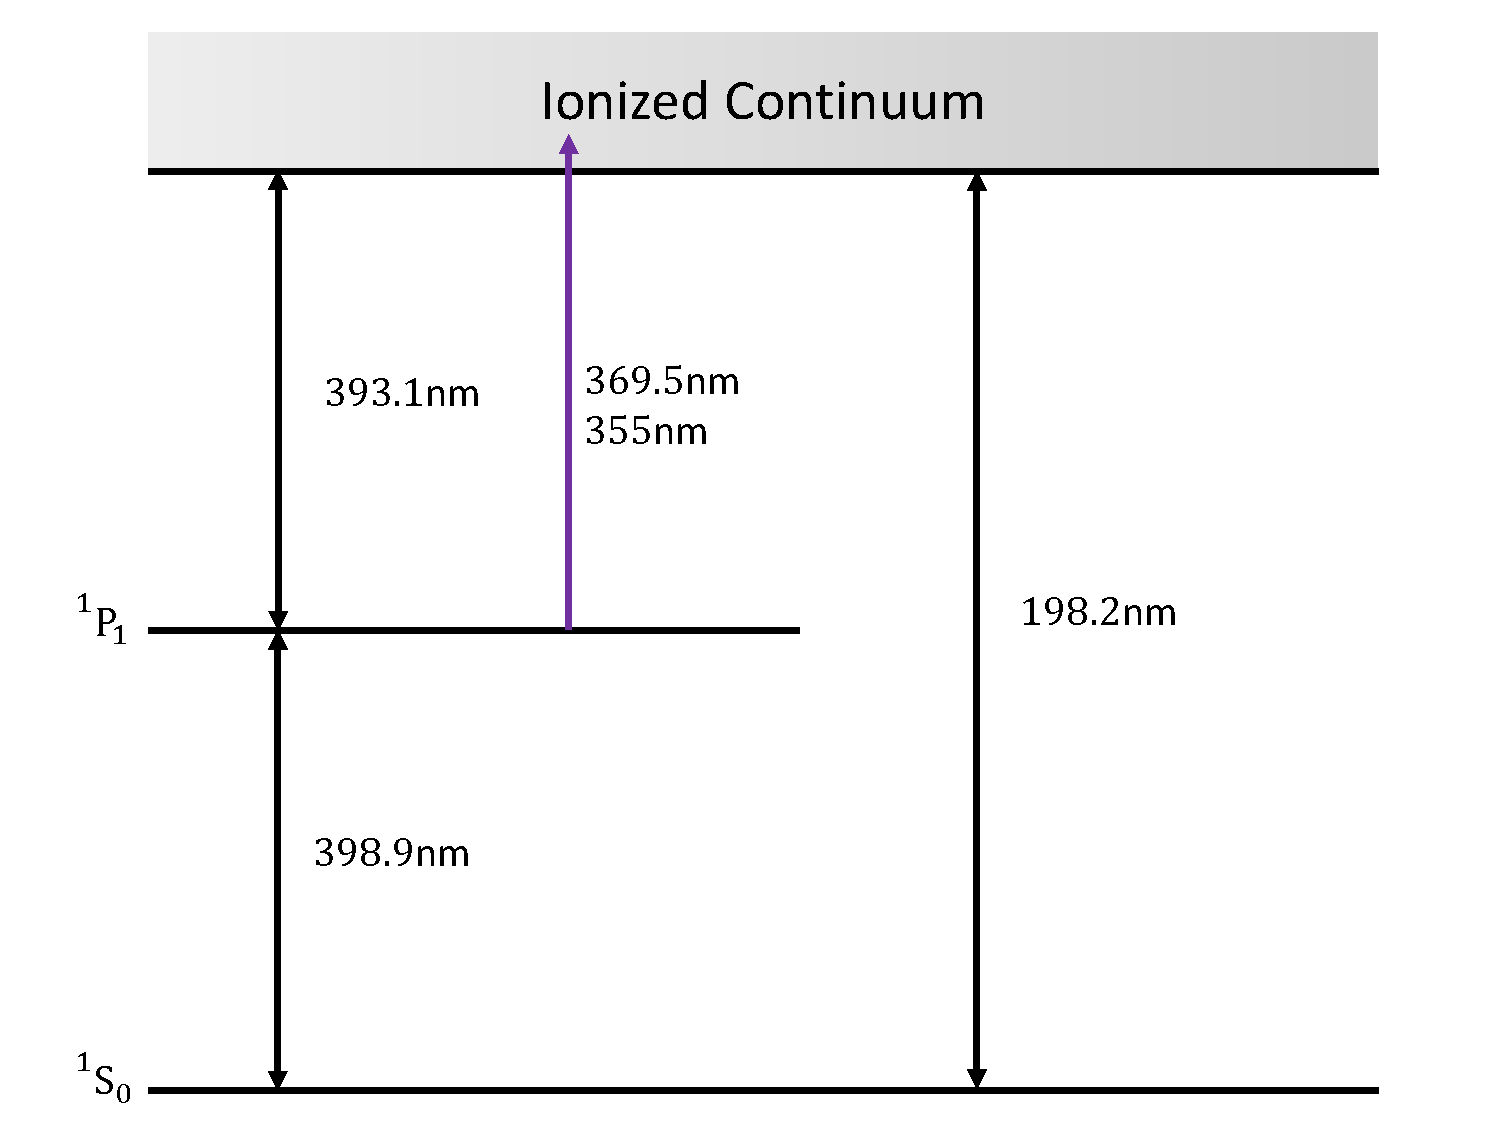
\includegraphics[width=0.5\linewidth]{fig_2_photo_ionization.pdf}
    \caption{Two-photon ionization scheme on ${ }^{171} \mathrm{Yb}^{+}$.}
    \label{fig:photo_ionization}
\end{figure}

Two-photon ionization allows for more precise control of isotope choice. The desired atomic source is often enriched, with an abundance as high as 91.7\%, the remainder consists of various natural isotopes, such as ${ }^{174} \mathrm{Yb}$, ${ }^{172} \mathrm{Yb}$, ${ }^{168} \mathrm{Yb}$ etc. Assume 50 ions in a large-scale trapped-ion quantum computer, and the average number of dark isotopes is 4. Thankfully, the intermediate level 398.91 nm transition exhibits an isotope-shift, which may be used to differentiate between isotopes. Doppler shift is a practical consideration that requires further care. The 398.91 nm laser is oriented perpendicular to the atomic flux to mitigate the Doppler effect. Isotope-selective loading of ions is possible in this setup, increasing the likelihood of the desired isotope, and this may be improved by decreasing the power of the 398.91 nm laser to achieve a narrow linewidth , although this might delay loading speed. Clock states, $\left|\downarrow_z\right\rangle \equiv\left|F=0, m_F=0\right\rangle$ and $\left|\uparrow_z\right\rangle \equiv\left|F=1, m_F=0\right\rangle$, encode the qubit. Doppler cooling, optical pumping and state detection all employ the cyclic transition between the $6^2 P_{1 / 2}$ states and the ground state $6^2 S_{1 / 2}$. A magnetic field applied externally causes a splitting of the $|F=1\rangle$ manifolds through the Zeeman effect at a rate of roughly 1.4 MHz/G, whereas the second-order Zeeman effect dominates the clock qubits at a rate of about 310 Hz/$\mathrm{G}^2$.

Routine ion loading procedures include directing an atomic beam to the loading zone, where several laser beams are utilized to photoionize the atoms. A needle and some shards of metal are all that make up the oven, enriched in 174Yb and 171Yb in separate ovens. On the outside, a current loop is created by connecting the needle's head and tail with Kapton wires to the positive and negative terminals of the power supply. No part of the needle should be anchored to the floor of the chamber. That's because doing so would generate a substantial current to flow into the ground. Since current flows preferentially toward a lower potential, this phenomena may be prevented by isolating the negative poles of the current source from the ground. Keep in mind that while powering the oven for the first time, we must increase the current gradually so as not to accidentally ignite it and safeguard the SAES pump. The first time you use an oven, numerous grimy items will likely be fired out, which might cause the SAES gauge current to rise to the order of A. The atoms are expelled into the trap's central zone after the oven is heated for several minutes.

\begin{figure}
    \centering
    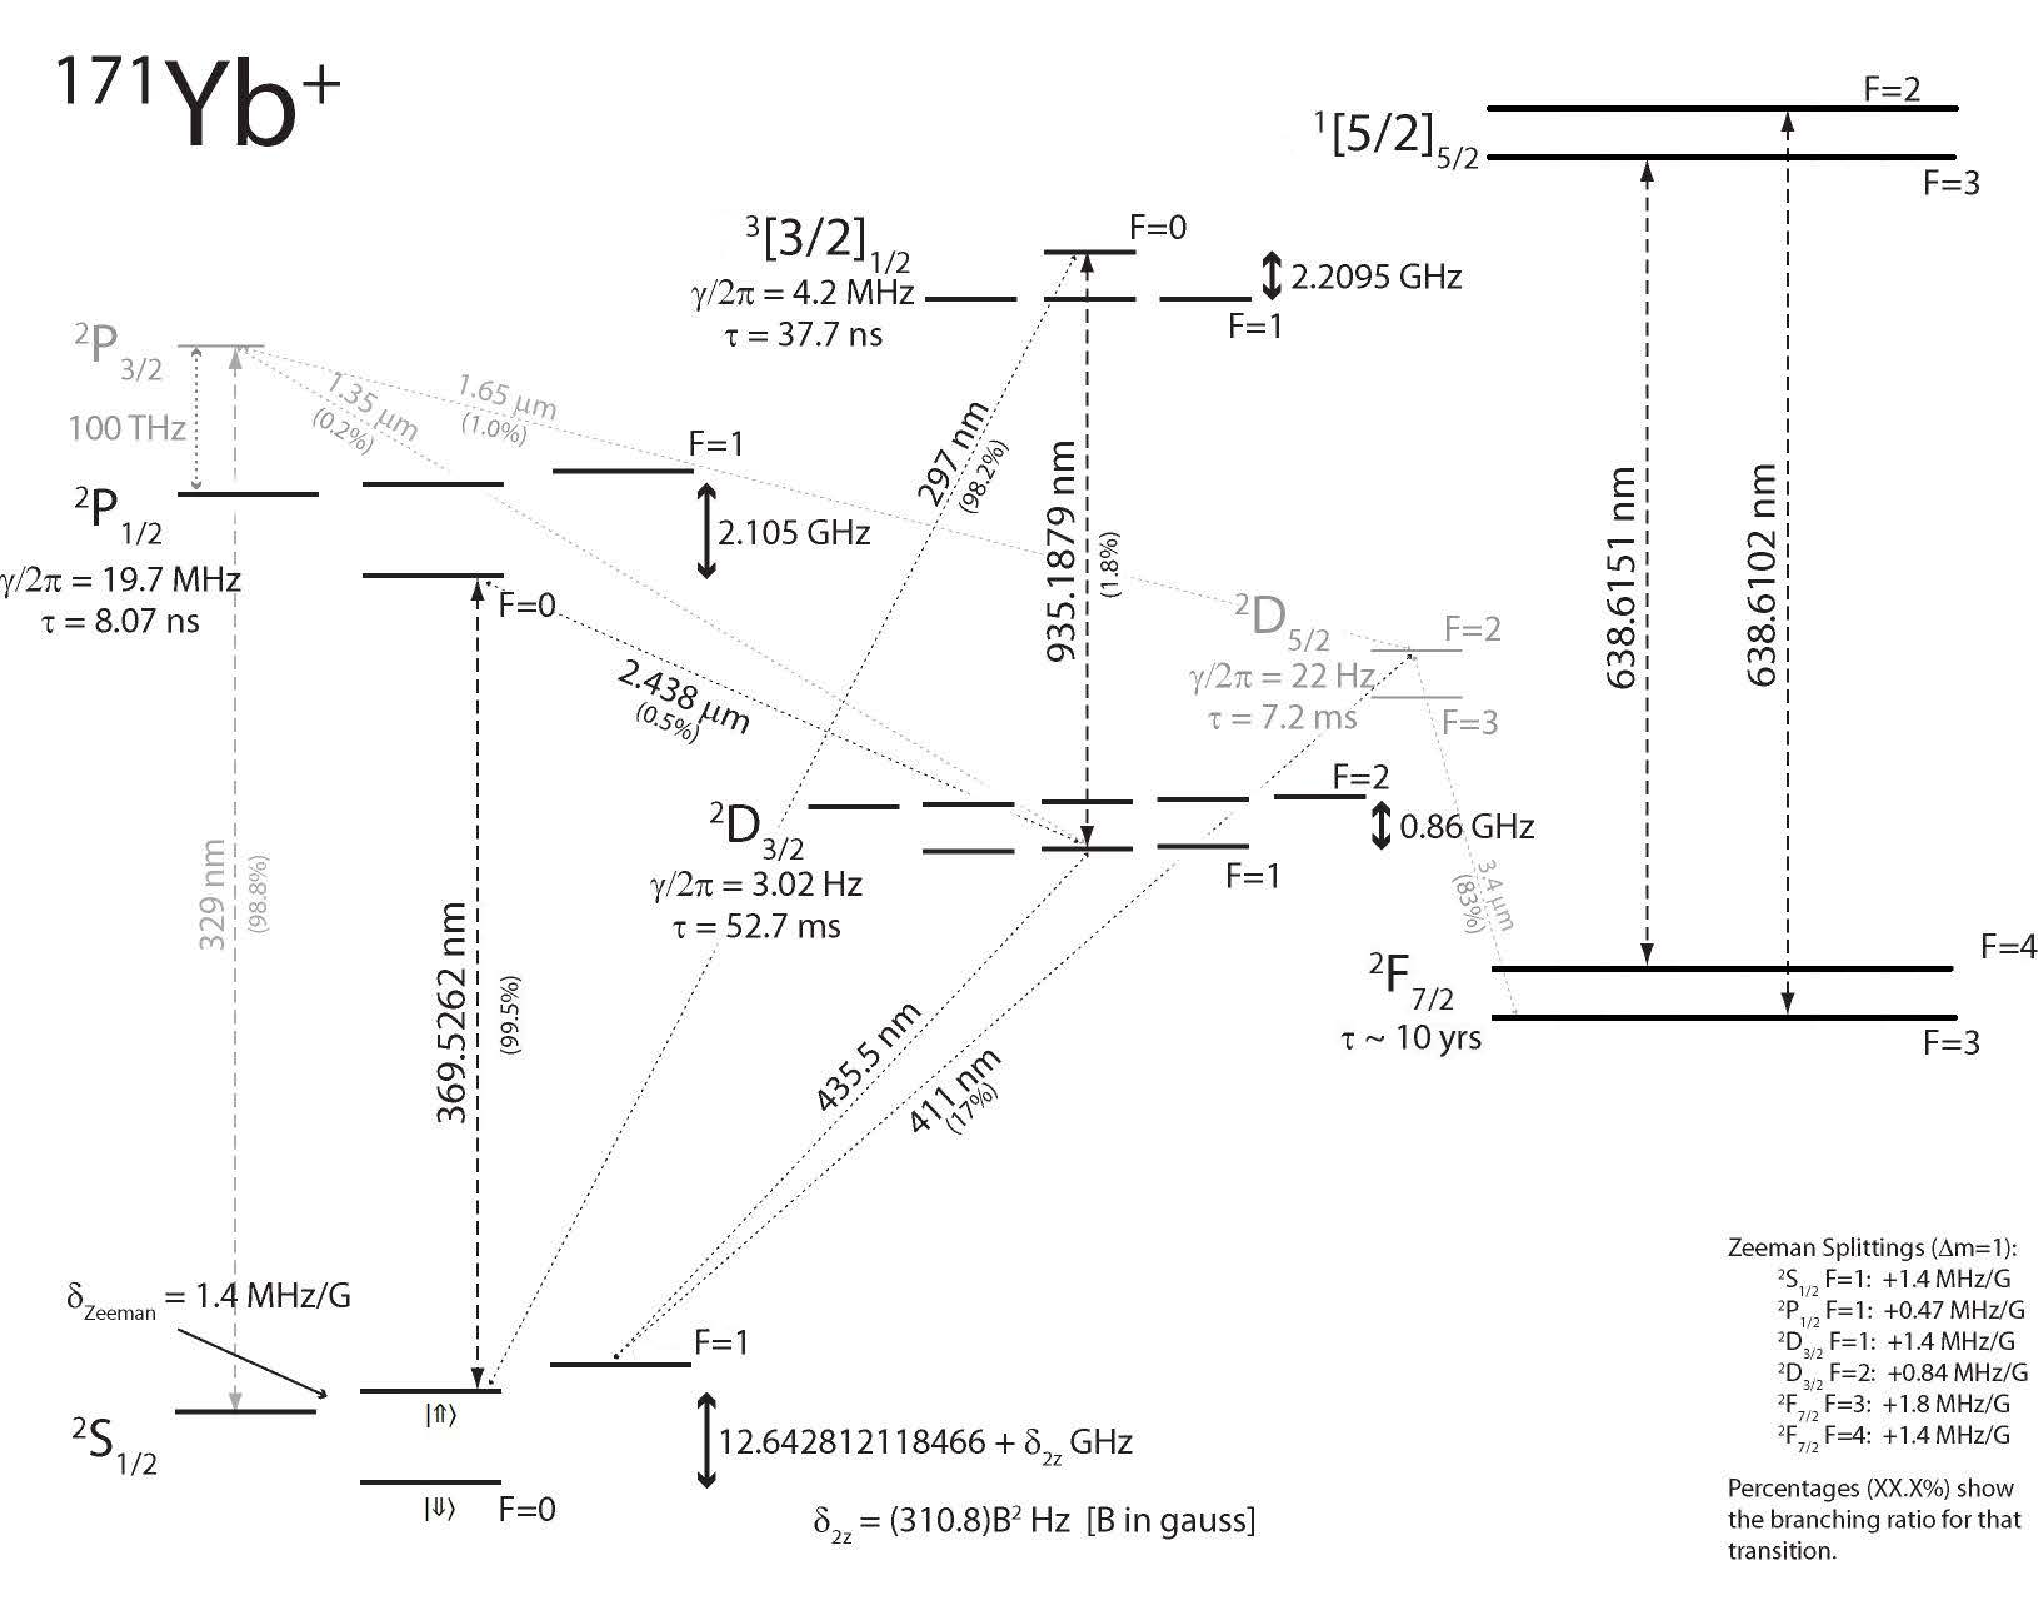
\includegraphics[width=1.0\linewidth]{fig_2_energy_level.pdf}
    \caption{${ }^{171} \mathrm{Yb}^{+}$ energy level diagram.}
    \label{fig:energy_level}
\end{figure}

\subsection{Doppler Cooling}

Ions have too wide of a motional area to be detected after they have been loaded into the trap since they are still very hot. We must first cool down the heated ions and produce the Coulomb crystal in order to stabilize and crystallize them. Doppler cooling is a method of rapidly cooling ions by utilizing a cyclic transition whose excited state has a very short lifetime and, therefore, a very high cooling rate. Doppler cooling is achieved in the ${ }^{171} \mathrm{Yb}^{+}$ system using a red-detuned laser to access $6^2 P_{1 / 2}$ levels with a lifetime of around 8.12 ns, a natural linewidth of 19.6 MHz, and a transition of 369.5263 nm.

Doppler cooling of ions is shown in a simplified model, where ion micromotion is disregarded and the trapping potential is represented by the time-independent pseudo harmonic potential $V(z)=\frac{1}{2} m \omega_z^2 z^2$ just in the z direction. Although the trapped ion's motion is no longer in the quantum domain after Doppler cooling, it can be treated as a classical motion with a velocity that obeys $v(t)=v_0 \cos \left(\omega_z t\right)$. Let us consider the hypothetical case of a single, moving laser interacting with a trapped two-level ion consisting only of S and P states. One cycle of absorption and spontaneous emission occurs in a time period where the ion's velocity does not vary noticeably if the radiative decay rateof the P-level is significantly bigger than the motional frequency. In this scenario, we may represent the average radiation pressure exerted on an ion as a continuous force that varies with its speed. A photon's absorption causes an ion's momentum to increase by $\Delta \mathbf{p}=\hbar \mathbf{k}$ in the direction of the photon's wave vector, and the ion's subsequent spontaneous emission likewise increases its momentum. After many cycles of absorption and emission, the ion will be slowed when the wave vector contains a component along the direction of motion, but the direction of the momentum kick due to spontaneous emission is random across cycles.

The Doppler cooling limit $T_{\min }=\hbar \Gamma(1+\chi) /\left(4 k_B\right)$ can be achieved by laser detuning $\Delta=-\frac{\Gamma}{2}$, where $\chi$ is the geometrical factor for spontaneous emission, $\Gamma=\sqrt{1+s} \Gamma_0$ is the effective linewidth broadened by power, $s$ is the saturation parameter and the saturation intensity is $I_{\text {sat }}=\frac{\pi h c \Gamma_0}{3 \lambda^3}=510 \mathrm{~W} / \mathrm{m}^2$. In addition, re-pumping $|\downarrow\rangle$ back to the cycled transition necessitates an additional frequency component with a detuning of 14.748 GHz. Moreover, the influence of the hyperfine levels must be taken into account, therefore a laser with a wavelength of 935.1880 nm and a sideband of 3.0695 GHz are needed. The branch ratio from level $6^2 P_{1 / 2}$ to level $5^2 D_{3 / 2}$ is non-zero at 0.5\%. Doppler cooling may be employed to achieve a final state with a phonon number below 10, where the crystal is stable against certain heating influences from the environment.

\begin{figure}
    \centering
    \subcaptionbox{Doppler cooling.}
    {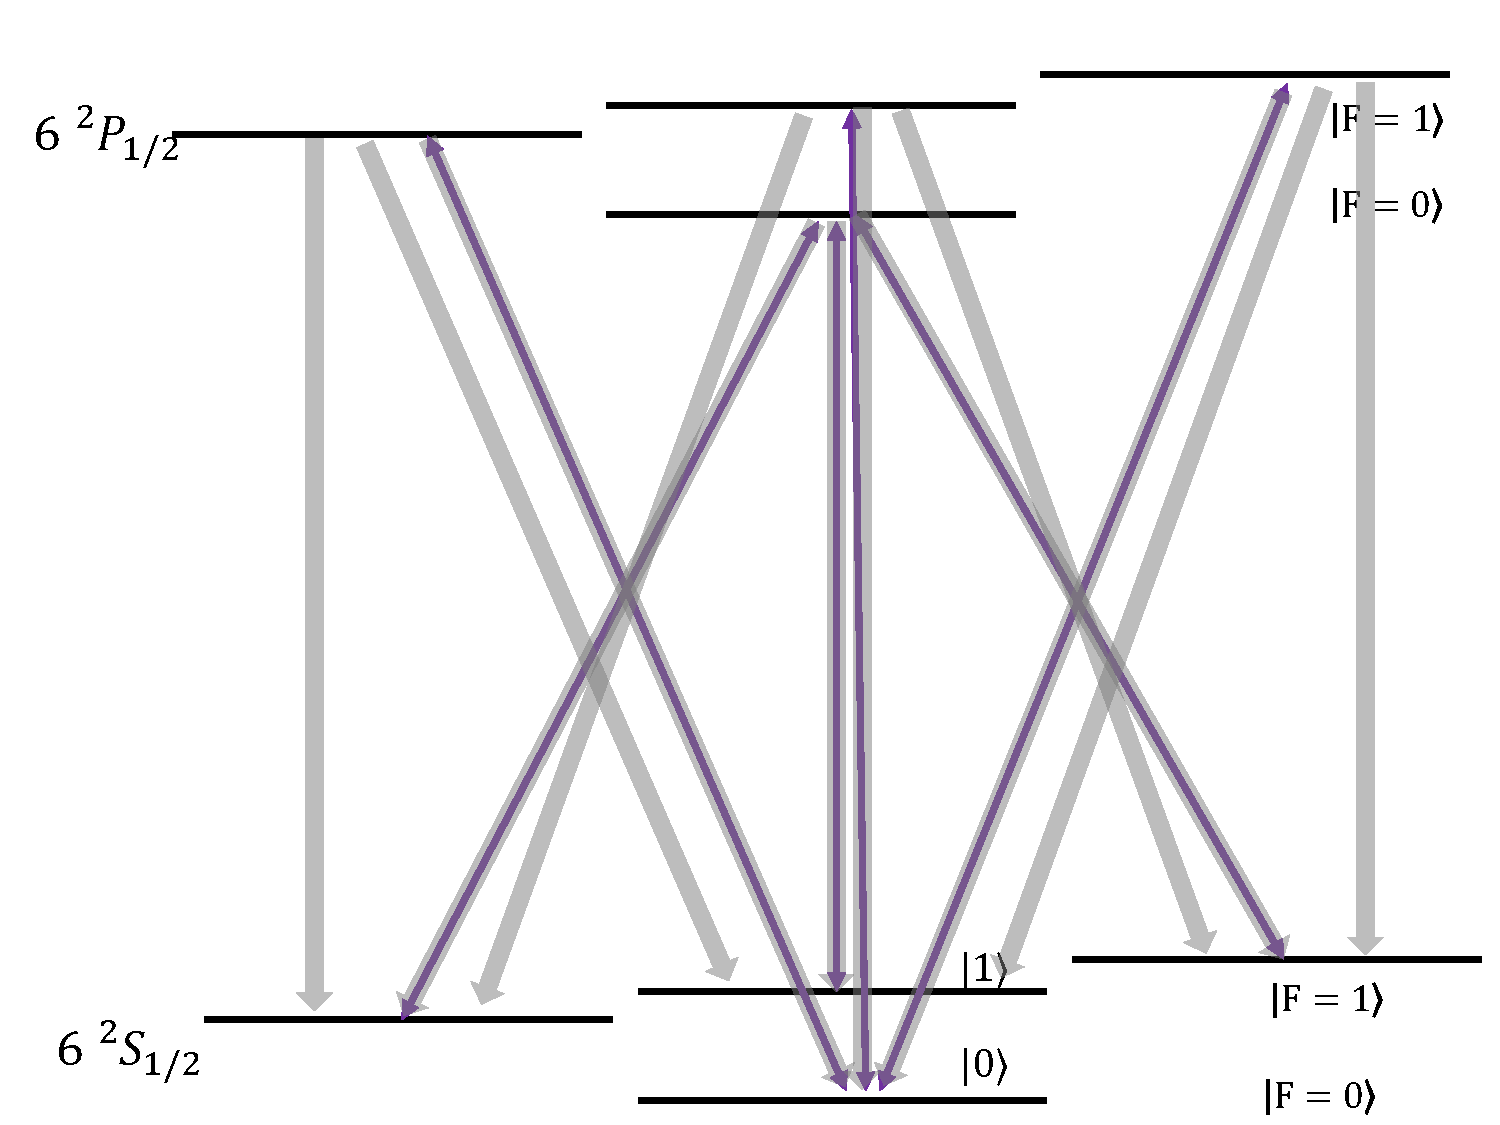
\includegraphics[width=0.4\linewidth]{fig_2_370_transitions_cooling.pdf}}
    \subcaptionbox{Optical pumping.}
    {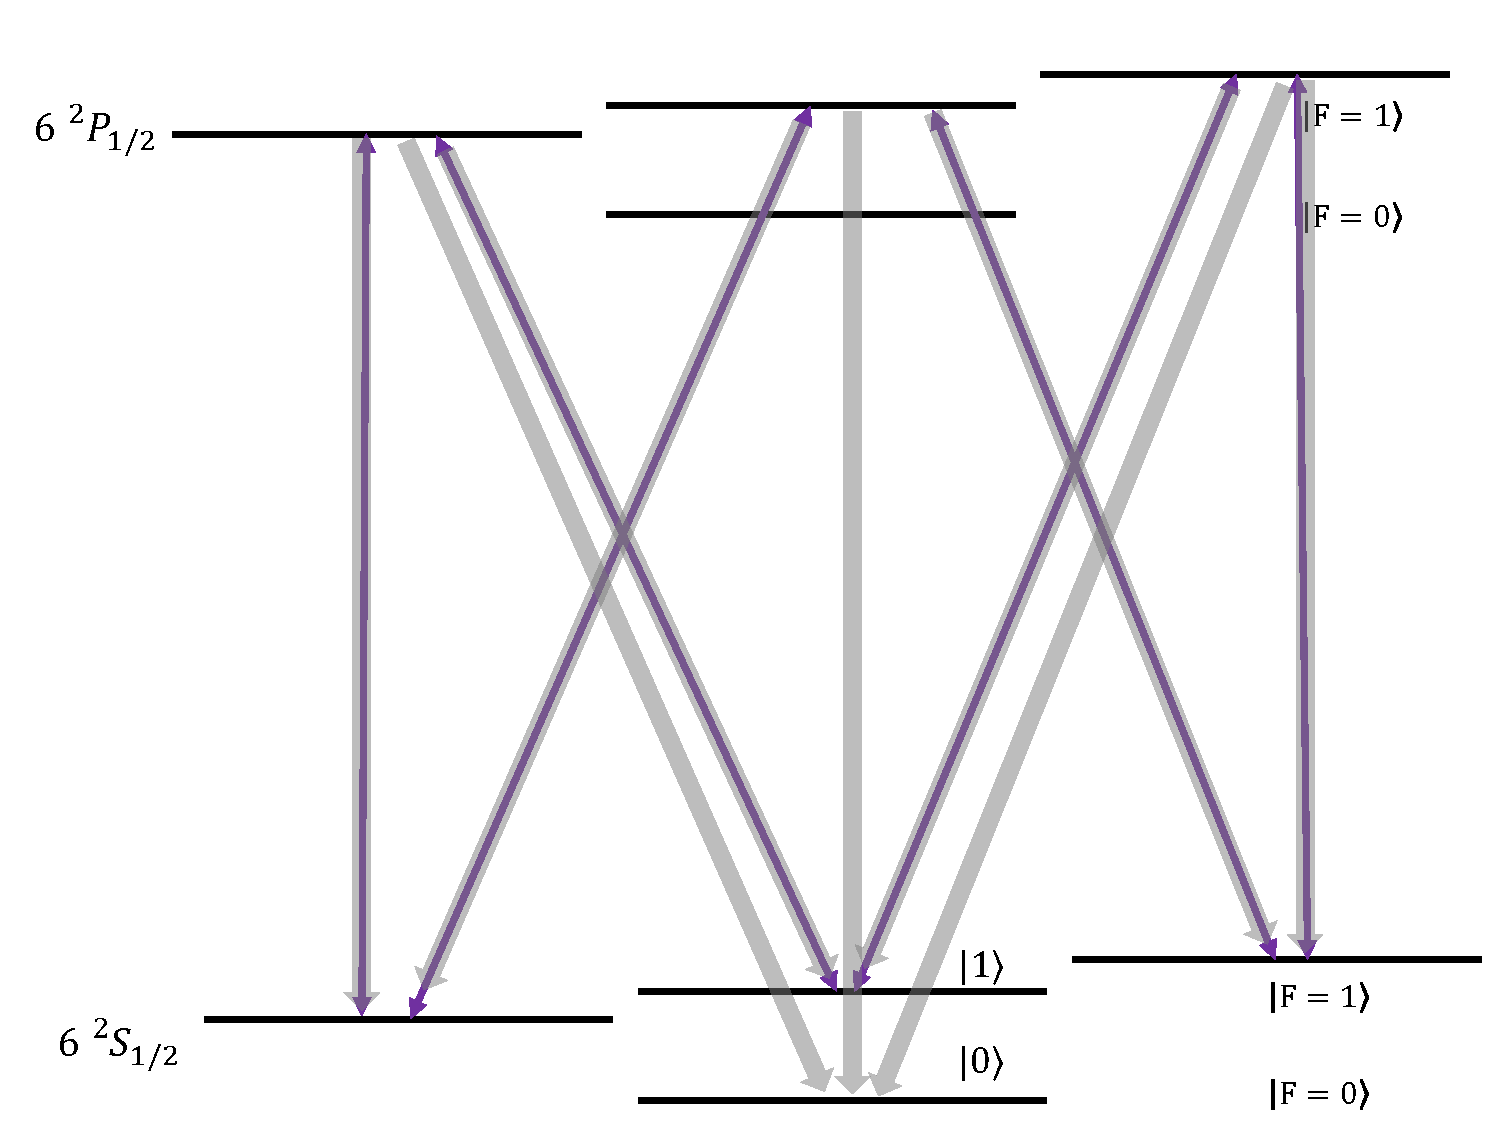
\includegraphics[width=0.4\linewidth]{fig_2_370_transitions_pumping.pdf}}
    \subcaptionbox{State detection.}
    {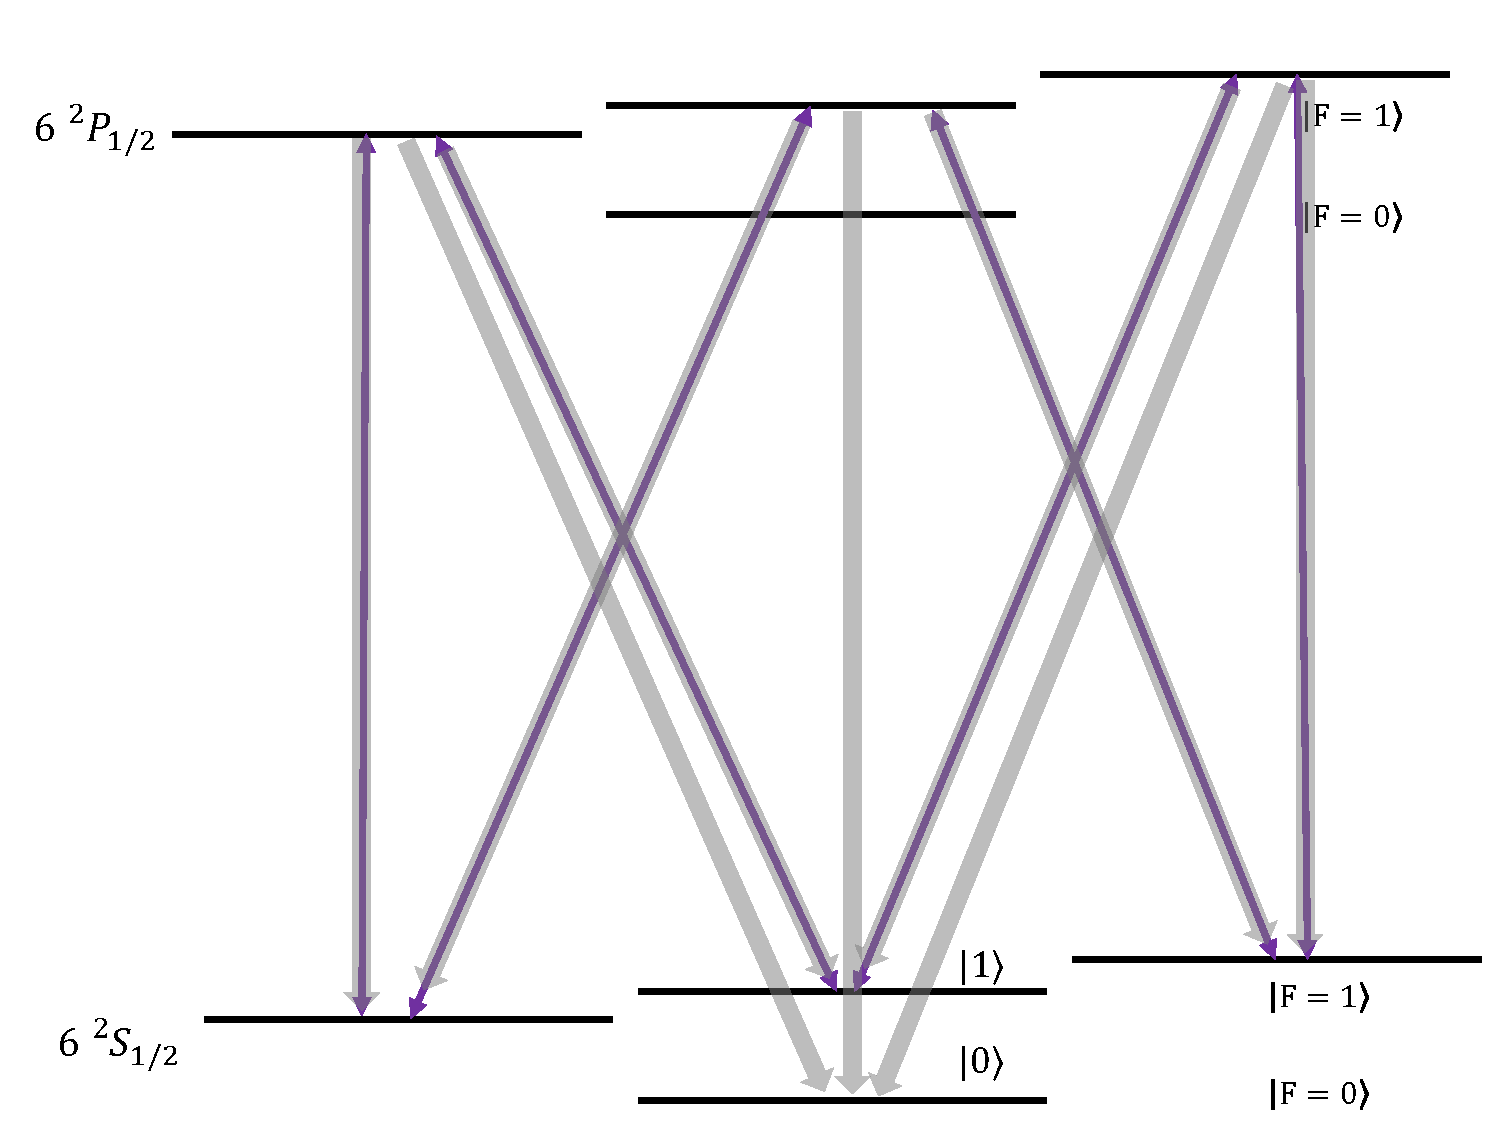
\includegraphics[width=0.4\linewidth]{fig_2_370_transitions_pumping.pdf}}
    \caption{The relevant transitions for 369.52 nm laser}
    \label{fig:370_transitions}
\end{figure}

\subsection{Optical Pumping}

When the ions have been cooled, the $\left|\downarrow_z\right\rangle$ state is prepared using optical pumping. Laser at 370 nm is stimulated when the ${ }^2 \mathrm{~S}_{1 / 2} \mathrm{~F}=1$ to ${ }^2 \mathrm{P}_{1 / 2} \mathrm{~F}=1$ transition occurs. If the ion enters the ${ }^2 \mathrm{P}_{1 / 2} \mathrm{~F}=1$ manifold, it may spontaneously decay to any of the ${ }^2 \mathrm{~S}_{1 / 2}$ states. The ion is $\sim$ 10GHz off resonant from the nearest transition. From the ${ }^2 \mathrm{P}_{1 / 2} \mathrm{~F}=1$ state, the ion has a 1/3 chance of decaying to the $\left|\downarrow_z\right\rangle$ state. According to the energy diagram, the optical pumping beam has to include both linear and circular components of polarization.

\subsection{State Detection}

An experiment's initial step is always preparing the $\left|\downarrow_z\right\rangle$ ion chain. The next step is to actually do the experiment, followed by analysis. When the $\hat{\sigma}_z$ operator is used for measurements, the $\left|\uparrow\right\rangle$ and $\left|\downarrow_z\right\rangle$ states of the ions are the only viable results.

It is possible to determine the state of the ion by shining light with a wavelength of 370 nm onto an ion chain that is resonant with the ${ }^2 \mathrm{~S}_{1 / 2} \mathrm{~F}=1$ to ${ }^2 \mathrm{P}_{1 / 2} \mathrm{~F}=0$ transition. This kind of light is known as a detecting light. The detecting light will only resonate with the $\left|\uparrow\right\rangle$ state if it is present. It is possible for the ion to decay spontaneously to any of the ${ }^2 \mathrm{~S}_{1 / 2} \mathrm{~F}=1$ levels. Since it is desirable to have numerous absorption or emission events, the beam has all possible polarization components. This allows the detection process to continue without interruption until sufficient photons have been gathered to determine the ion state. The ion fluoresces isotropically when exposed to the detecting light, and a portion of the light that is emitted by it is gathered by imaging optics and directed onto an EMCCD camera in order to read out the spin state. The detection light has a minuscule chance of off-resonantly exciting either spin state to the ${ }^2 \mathrm{P}_{1 / 2} \mathrm{~F}=1$ manifold, where the ion may subsequently decay into the other spin state and induce detection errors. This happens because of the ${ }^2 \mathrm{P}_{1 / 2} \mathrm{~F}=1$ manifold.

Doppler cooling, optical pumping, and state detection are all examples of operations that entail spontaneous decay to the ${ }^2 \mathrm{~S}_{1 / 2} \mathrm{~F}=1$ manifold of states. Hence, if the Zeeman states are degenerate, the mechanism of coherent population trapping may be used to pump the ion into a dark state. As a result, an application of a B-field is made to the ions in order to disrupt this degeneracy and stop the trapping of coherent populations. In the location where the ions are located, the B-field strength is XX G, and the Zeeman splitting from the $\left|\uparrow\right\rangle$ state is measured XX MHz.

We are able to determine the state of the spins in the ion chain by capturing the spin-dependent fluorescence using a site-resolving image Andor IXon Ultra 888 EMCCD camera. During the state detection process, a resonant laser with a wavelength of 370 nm is shone between $\left|\uparrow\right\rangle$ and $\left|\downarrow_z\right\rangle$. When the qubit is in the $\left|\downarrow_z\right\rangle$ state, a small amount of photons are scattered off, however when the spin state is in the $\left|\uparrow\right\rangle$ state, a significant number of photons are scattered off. The binary threshold for spin-state discrimination is determined by calibrating the number of photons dispersed from the bright $\left|\uparrow\right\rangle$ state and the dark $\left|\downarrow_z\right\rangle$ state of each spin at the beginning of the process of collecting data on those spins. The bright and dark states of the setup used in this thesis have an average fidelity of more than 97 \%, which is suitable for the quantum memory experiments. The off-resonant mixing of spin states during detection, crosstalk between nearby ions, noise from the electronic camera, and noise from the laser are the primary causes of mistake in this case.


\section{The Linear Paul Trap}

According to one of Maxwell's equations, $\nabla \cdot \vec{E}=0$, the electric field will not diverge in a region where there is no free charge density. This conclusion may be drawn from the fact that: Earnshaw deduced from this equation that it was mathematically impossible for a charged particle to be connected in a static electric field in all directions at the same time. Yet, in order to condense charged particles, either oscillating electric fields or a combination of static electric and magnetic fields are required. In this experiment, the RF trap is the primary focus.

Assuming for the sake of this discussion that the ions have a positive charge, mathematically express the criteria of an accessible potential that requires minima in any direction as shown below.

\begin{equation}\label{eq:minima}
    \frac{\partial \mathbf{E}}{\partial x_i}=-\frac{\partial^2 \Psi}{\partial x_i^2}<0, x_i \in\{x, y, z\}
\end{equation}

However, Eq.~\eqref{eq:minima} contradicts of the Laplacian equation for static electric fields in vacuum, which states that else there would never be a global minimum in any of the directions otherwise $\frac{\partial \mathbf{E}}{\partial x_i}=0$

\begin{equation}
    \nabla^2 \Psi=0
\end{equation}


The ion trap technique, which uses a mix of DC and RF oscillating electric fields, offers a fortunate alternative to the traditional method of confining ions in a vacuum environment. It is possible to write down the broad potential of a Paul trap as

\begin{equation}\label{eq:rfpotential}
    \Psi(x, y, z)=\frac{U}{2}\left(\alpha x^2+\beta y^2+\gamma z^2\right)+\frac{V}{2} \cos (\Omega t)\left(\alpha^{\prime} x^2+\beta^{\prime} y^2+\gamma^{\prime} z^2\right)
\end{equation}

$\alpha, \beta, \gamma, \alpha^{\prime}, \beta^{\prime}, \gamma^{\prime}$ are geometrical factors. A potential of this kind may be generated using hyperbolic electrodes, the geometrical factors involved are precisely $1 / r^2$, where $r$ denotes the distance to the electrodes. Unfortunately, the hyperbolic electrodes restrict the optical access. There are some novel designs for traps with high optical access, but the geometrical considerations need to take into account the approximations that are necessary since the hyperbolic electrodes are not ideal. There is an extra restriction for the geometrical factors that must be satisfied in order to satisfy the Laplacian equation

\begin{equation}
    \alpha+\beta+\gamma=0,\quad \alpha'+\beta'+\gamma'=0
\end{equation}

To be more specific, a Paul trap with the parameters $\gamma^{\prime}=0, \alpha=\beta=-\frac{\gamma}{2}, \alpha^{\prime}=-\beta^{\prime}$ is referred to as a linear trap. In a linear trap, charged particles are only confined by a static field in one direction, while RF fields are used to confine them in the other two directions.

\subsection{Mathieu Equation}

With a Paul trap, it is possible to decouple the motion of charged particles in three different directions. In this case, we will treat in $x$ for the sake of simplicity following,

\begin{equation}\label{eq:motion}
    m \frac{\mathrm{d}^2 x}{\mathrm{~d} t^2}=-Q\left(\alpha U x+\alpha^{\prime} V \cos (\Omega t) x\right)
\end{equation}
substitute $\tau=\frac{\Omega t}{2}, a_x=\frac{4 Q U \alpha}{m \Omega^2}, q_x=\frac{2 Q V \alpha^{\prime}}{m \Omega^2}$, Eq.~\eqref{eq:motion} can be simplified as a Mathieu equation

\begin{equation}
    \frac{\mathrm{d}^2 x}{\mathrm{~d} \tau^2}+\left(a_x x-2 q_x \cos (2 \tau) x\right)=0
\end{equation}

In this case, the solution of the lowest order is shown together with the assumptions that $\left|a_x\right|, q_x^2 \ll 1$,

\begin{equation}
    \beta_x=\sqrt{a_x+\frac{q_x^2}{2}}, \quad x(t)=2 A C_0 \cos \left(\beta_x \frac{\Omega t}{2}\right)\left[1-\frac{q_x}{2} \cos (\Omega t)\right]
\end{equation}

This is a bounded solution with periodic frequency $\omega_x=\frac{\beta_x \Omega}{2}$, which is often referred to as secular motion. The second component in frequency $\Omega \pm \omega_x$ represents the intrinsic micromotion that is induced by the RF fields.

In a further approximation, it is possible to construct an effective time-independent potential to describe the dynamics of charged particles in an RF Paul trap. An example in $x$ is presented below, and we assume that the charge is equal to $e$.

\begin{equation}
    E(x, t)=E_0(x) \cos (\Omega t)
\end{equation}

\begin{equation}
    F(x, t)=m \ddot{x}=e E_0(x) \cos (\Omega t)
\end{equation}

where $E_0(x)$ is independent of the time-varying potential and solely depends on positional information. Imagine a crystal that has been stabilized such that all of its ions remain in close proximity to their positions of equilibrium. The only new vibrations that occur are those that are caused by the RF fields.

\begin{equation}\label{eq:staticmotion}
    x=x_0-\frac{eE_0(x_0)}{m\Omega^2}\cos(\Omega t)
\end{equation}

This is the first-order solution to the motion, and we may do additional Taylor expansion at the equilibrium location $x_0$ to the electric field as well, although this is not necessary.

\begin{equation}
    \begin{aligned}
        E_0(x) & =E_0\left(x_0\right)+\left.\frac{\partial E_0(x)}{\partial x}\right|_{x_0}\left(x-x_0\right)                                                    \\
               & =E_0\left(x_0\right)-\left.\frac{\partial E_0(x)}{\partial x}\right|_{x_0}\left(\frac{e E_0\left(x_0\right)}{m \Omega^2} \cos (\Omega t)\right) \\
               & =E_0\left(x_0\right)-\left.\frac{e}{2 m \Omega^2} \frac{\partial E_0^2(x)}{\partial x}\right|_{x_0} \cos (\Omega t)
    \end{aligned}
\end{equation}

\begin{equation}
    \begin{aligned}
        F(x, t)=m \ddot{x} & =e E_0\left(x_0\right) \cos (\Omega t)-\left.\frac{e^2}{2 m \Omega^2} \frac{\partial E_0^2(x)}{\partial x}\right|_{x_0} \cos ^2(\Omega t)        \\
                           & =e E_0\left(x_0\right) \cos (\Omega t)-\left.\frac{e^2}{2 m \Omega^2} \frac{\partial E_0^2(x)}{\partial x}\right|_{x_0}(1+\cos (2 \Omega t)) / 2
    \end{aligned}
\end{equation}

Assess the influence on average, excluding out the variables that are rapidly fluctuating,

\begin{equation}
    \bar{F}(x)=-\left.\frac{e^2}{4 m \Omega^2} \frac{\partial E_0^2(x)}{\partial x}\right|_{x_0}
\end{equation}

where \(E_0(x)=-\alpha'V x\) for the general potential, it is a harmonic confinement that does not rely on whether the ions are positively or negatively charged, and it controls the secular motion of ions inside the trap. Additional words include the source of micromotion, which has an oscillation that is much more rapid and is defined by frequency \(\Omega\). Hence, one way to define the pseudo potential is as follows,

\begin{equation}\label{eq:pseudo_potential}
    \Psi_{ps}=\frac{e}{4m\Omega^2}E_0^2(x)=\frac{e\alpha'^2V^2}{4m\Omega^2}x^2
\end{equation}

This re-creates the conclusion that Earnshaw's theorem came to. It is a valid approximation for equilibrium positions and secular motion of charged particles in an RF trap, and it can be used to calculate the principal axes taking both DC and RF fields into account. The secular frequency is \(\omega_x=\frac{e\alpha' V}{\sqrt{2}m\Omega}\), which is consistent with the Mathieu equation. The static confinement can also be taken into account, which is also a harmonic term.

\subsection{Normal Modes}

Since the normal modes are entirely decoupled from all directions, particularly the transverse modes that we are working on, we employ a chain of trapped ${ }^{171} \mathrm{Yb}^{+}$ ions as the quantum memory in a linear Paul trap. This allows us to study the transverse modes. It is necessary for the trap frequencies to adhere to the relation Eq.~\eqref{eq:linear_chain} if the Coulomb crystal is to be contained inside a linear chain.

\begin{equation}\label{eq:linear_chain}
    \left(\frac{\omega_r}{\omega_z}\right)^2 \geq \frac{N^{1.73}}{2.53}
\end{equation}

where \(N\) is the number of ions, \(\omega_r\) refers to either the transverse mode \(\omega_x\) or \(\omega_y\), and \(\omega_z\) refers to the axial mode with DC confinement.

Instead of using the straightforward Mathieu equation, one needs take into consideration the Coulomb interaction that occurs between the ions when there are a greater number of ions fed into the trap. Both the externally imposed pseudo potential and the Coulomb interactions that occur between the ions work together to decide the shape of the ion crystal.

The inter-ion spacings would not be uniform under a harmonic potential similar to Eq.~\eqref{eq:rfpotential}, where spacings at the center of an ion chain would be much more tight but loose at the edge. This would require much higher RF potential or lower DC potential to satisfy Eq.~\eqref{eq:linear_chain}, or else there would be an unstable transition to zigzag mode. Here, we consider \(N\) ions in In order to solve the issue, quartic potential is required. This is because increasing the number of electrodes along the z-axis will bring the inter-ion spacings closer to being uniform. As the micromotion is negligible in comparison to the secular motion and all of the ions are aligned with the RF null in the required configuration, the property of the ion crystal may be obtained using the pseudo potential while ignoring the time-dependent RF potential.

The potential in its broadest sense may be expressed as

\begin{equation}
    U=\sum_i\left(\frac{\alpha}{2} z_i^2+\frac{\beta}{4} z_i^4\right)+\sum_{i<j} \frac{e^2}{4 \pi \epsilon_0\left|z_i-z_j\right|}
\end{equation}

Here, we will define the length unit known as \(l=\qty(e^2/4\pi\epsilon_0\alpha)^{1/3}\), and after that, we will be able to rewrite the potential \(u_i\equiv z_i/l\) using dimensionless coordinates and dimensionless energy \(U'\equiv 4\pi \epsilon_0 lU/e^2\), respectively.

\begin{equation}\label{eq:dimensionlessaxialpotential}
    U'=\sum_i\qty(\frac{1}{2}u_i^2+\frac{\beta l^2}{4\alpha}u_i^4)+\sum_{i\ne j}\frac{sgn(\alpha)}{2\abs{u_i-u_j}}
\end{equation}\

where \(sgn(x)\) is the sign function.

% Once we have determined the ion number and the potential configuration \(\frac{\beta l^2}{\alpha}\), we can minimize the energy to find the equilibrium positions. Alternatively, we can solve the equations of gradient at equilibrium
% \begin{equation}\label{eq:gradient}
%     0=\pdv{U'}{u_i}=u_i+\frac{\beta l^2}{\alpha}u_i^3-sgn(\alpha)\sum_{i\ne j}\frac{u_i-u_j}{\abs{u_i-u_j}^3}
% \end{equation}

% Rather than perform the optimization with multiple variables, we can further reduce the problem to find the solutions of the gradient equations, which can be easily accomplished by some built-in functions of Wolfram Mathematica such as FindRoot or NSolve.

% After obtaining the equilibrium positions, the axial motional modes can be computed by the Hessian matrix
% \begin{equation}\label{eq:axial_hessian}
%     \pdv{U'}{u_i}{u_j}=\begin{cases}
%         1+\frac{3\beta l^2}{\alpha}u_i^2+\sum_{k\ne i}\frac{2sgn(\alpha)}{\abs{u_i-u_k}^3}, & i=j    \\
%         -\frac{2sgn(\alpha)}{\abs{u_i-u_j}^3},                                              & i\ne j
%     \end{cases}
% \end{equation}

% To show a brief picture of the potential, we will give an example based on our BEM simulation of \(5\)-segment blade trap(See Sec.~\ref{sec:idealpotential}). For a harmonic potential \(\alpha> 0\), we can set the voltage of DC segments as \(\qty(1,\,0,\,0,\,0,\,1)\,\unit{V}\), the simulated results of \(60\) \yb{171} ions are shown in Fig.~\ref{fig:harmonic}, the length of the ion chain is about \(200\,\unit{\um}\), the lowest center-of-mass(COM) mode is \(92.76\,\unit{\kHz}\) and the potential depth by \(\pm 150\,\unit{\um}\) is about \(0.0065\,\unit{eV}\), and the inter-ion spacings are increasing from the center to the edge with a relative standard deviation(RSD) \(28.4\%\). For such a configuration, the repulsion among the central ions would be strongest and thus the zigzag transition would first take place in the center, which could be avoided by lowering the axial confinement or increasing the RF confinement.

% \begin{figure}[hbtp]
%     \centering
%     \subcaptionbox{}[0.5\linewidth]{\includegraphics[width=\linewidth]{harmonic_potential.pdf}}\hfill
%     \subcaptionbox{}[0.5\linewidth]{\includegraphics[width=\linewidth]{harmonic_spacing.pdf}}
%     \caption[Equilibrium positions and ion spacings in the harmonic potential]{\label{fig:harmonic}(a) The equilibrium positions, (b) The inter-ion spacings of \(60\) \yb{171} ions in the harmonic potential, the relative standard deviation(RSD) is \(28.4\%\).}
% \end{figure}

% However, we have two degrees of freedom for the axial confinement so that we can engineer a quartic potential \(\alpha<0,\,\beta>0\), the voltages can be set \(\mqty(10&0&2.4&0&10)\,\unit{V}\) to achieve the same size of \(60\)-ion crystal in length of \(200\,\unit{\um}\), typically the COM mode frequency would be higher than the harmonic one and here it is \(95.57\,\unit{\kHz}\). The potential depth by \(\pm 150\,\unit{\um}\) is about \(0.0125\,\unit{\eV}\) and the inter-ion spacings are much more uniform with RSD \(11.9\%\), which can be further improved if we have more DC electrodes. In addition, the bandwidth of the normal modes can be narrower for quartic potential, as seen in Fig.~\ref{fig:narrow_bandwidth}, this would enable us a better control over the normal modes such as the ground state cooling. The corresponding \(60\) dimensionless normal mode vectors are depicted as in Fig.~\ref{fig:axial_modes}, the mode structure is completely different that modes are distributed more uniformly for quartic potential and the strengths of normal mode vectors represent the contribution for specific normal modes.
% \begin{figure}[hbtp]
%     \centering
%     \subcaptionbox{}[0.5\linewidth]{\includegraphics[width=\linewidth]{quartic_potential.pdf}}\hfill
%     \subcaptionbox{}[0.5\linewidth]{\includegraphics[width=\linewidth]{quartic_spacing.pdf}}
%     \caption[Equilibrium positions and ion spacings in the quartic potential]{\label{fig:quartic}(a) The equilibrium positions, (b) The inter-ion spacings of \(60\) \yb{171} ions in the quartic potential, the relative standard deviation(RSD) is \(12.0\%\)}
% \end{figure}

% \begin{figure}[hbtp]
%     \centering
%     \subcaptionbox{Harmonic potential.}[0.5\linewidth]{\includegraphics[width=\linewidth]{harmonic_freq.pdf}}\hfill
%     \subcaptionbox{Quartic potential.}[0.5\linewidth]{\includegraphics[width=\linewidth]{quartic_freq.pdf}}
%     \caption[The axial normal mode frequencies]{\label{fig:narrow_bandwidth}The axial normal mode frequencies of \(60\) \yb{171} ions in two kinds of potential form.}
% \end{figure}

% \begin{figure}[hbtp]
%     \centering
%     \subcaptionbox{Harmonic potential.}[0.5\linewidth]{\includegraphics[width=\linewidth]{harmonic_axial_mode.pdf}}\hfill
%     \subcaptionbox{Quartic potential.}[0.5\linewidth]{\includegraphics[width=\linewidth]{quartic_axial_mode.pdf}}
%     \caption[The axial normal mode vectors]{\label{fig:axial_modes}The dimensionless normal mode vectors along trap axis of \(60\) \yb{171} ions in two kinds of potential form, the mode index starts from the lowest COM mode and the strengths of mode vectors represent the contribution to specific modes.}
% \end{figure}

% As for the transverse modes, things would be different. The COM mode is the highest one and the bandwidth is near the axial COM mode\cite{zhu2006trapped}, thus the transverse modes are much more crowded. We can further include the transverse terms in a general form
% \begin{equation}\label{eq:allpotential}
%     U=\sum_i\qty(\frac{\alpha}{2}z_i^2+\frac{\beta}{4}z_i^4+\frac{1}{2}m\omega_x^2x_i^2+\frac{1}{2}m\omega_y^2y_i^2)+\sum_{i<j}\frac{e^2}{4\pi\epsilon_0\abs{\vb{r_i}-\vb{r_j}}}
% \end{equation}

% For a linear chain configuration, the equilibrium positions for transverse \(x,\, y\) are quite clear that \(x_0=0,\,y_0=0\), and we can use the same dimensionless unit \(l\) to simplify the potential expression using notation \(uz=z/l,\, ux=x/l,\, uy=y/l\),
% \begin{equation}\label{eq:dimensionlesspotential}
%     \begin{aligned}
%         U' & =\sum_i\qty(\frac{1}{2}uz_i^2+\frac{\beta l^2}{4\alpha}uz_i^4+\frac{m\omega_x^2}{2\alpha}ux_i^2+\frac{m\omega_y^2}{2\alpha}uy_i^2)+\sum_{i\ne j}\frac{sgn(\alpha)}{2\abs{\vb{u_i}-\vb{u_j}}} \\
%            & =U_0+\sum_i\qty(\frac{m\omega_x^2}{2\alpha}ux_i^2+\frac{m\omega_y^2}{2\alpha}uy_i^2)-sgn(\alpha)\sum_{i\ne j}\frac{\qty(ux_i-ux_j)^2+\qty(uy_i-uy_j)^2}{4\abs{uz_i-uz_j}^3}
%     \end{aligned}
% \end{equation}
% where \(U_0\) is the one only related to coordinates \(uz_i\)'s, and we can neglect them without loss of generality when considering the transverse modes. We can also obtain the Hessian matrix for \(x,\, y\), and the results for \(x\) is present below, and RHS of the potential has the same dependence on the sign of \(\alpha\), in practice, we can directly use the absolute value,

% \begin{equation}\label{eq:transverse_hessian}
%     \pdv{U'}{ux_i}{ux_j}=\begin{cases}
%         \frac{m\omega_x^2}{\abs{\alpha}}-\sum_{k\ne i}\frac{1}{\abs{uz_i-uz_k}^3}, & i=j    \\
%         \frac{1}{\abs{uz_i-uz_j}^3},                                               & i\ne j
%     \end{cases}
% \end{equation}

% Here, we show an example of the above crystal, and set the transverse trap frequency as \(2\pi \times 2.47\,\unit{\MHz}\), clearly the transverse mode bandwidth is narrower for the quartic potential as shown in Fig.~\ref{fig:transverse_freq}, once the zigzag mode frequency is low and then the transition probability to a 2D zigzag pattern would be high.  In particular, the mode vectors are in a way the inverse of the axial one, as we can see in Fig.~\ref{fig:axial_modes} and Fig.~\ref{fig:transverse_modes}.
% \begin{figure}[hbtp]
%     \centering
%     \subcaptionbox{Harmonic potential.}[0.5\linewidth]{\includegraphics[width=\linewidth]{transverse_harmonic_freq.pdf}}\hfill
%     \subcaptionbox{Quartic potential.}[0.5\linewidth]{\includegraphics[width=\linewidth]{transverse_quartic_freq.pdf}}
%     \caption[The transverse normal mode frequencies]{\label{fig:transverse_freq}The transverse normal mode frequencies of \(60\) \yb{171} ions in two kinds of potential form.}
% \end{figure}

% \begin{figure}[hbtp]
%     \centering
%     \subcaptionbox{Harmonic potential.}[0.5\linewidth]{\includegraphics[width=\linewidth]{transverse_harmonic_mode.pdf}}\hfill
%     \subcaptionbox{Quartic potential.}[0.5\linewidth]{\includegraphics[width=\linewidth]{transverse_quartic_mode.pdf}}
%     \caption[The transverse normal mode vectors]{\label{fig:transverse_modes}The dimensionless normal mode vectors along transverse axes of \(60\) \yb{171} ions in two kinds of potential form, the mode index starts from the lowest zigzag mode and the strengths of mode vectors represent the contribution to specific modes.}
% \end{figure}



\section{notation}

${ }^{171} \mathrm{Yb}^{+}$

$6^2 P_{1 / 2}$

$|\downarrow\rangle$

$\left|\downarrow_z\right\rangle$

$\left|\uparrow\right\rangle$

